\dev{Emile Martinez}{}

La théorie des jeux s'intéresse aux interactions entre des individus (joueurs) qui effectuent des choix selon les règles d'un jeu.

\section{Jeux d'accessibilité à deux joueurs}

\subsection{Définition}

\paragraph{Notation :} Pour $G = (S, A)$, on note $Fin(G) = \{v \in S / deg^+(v) = 0\}$

\begin{definition}
	\label{16-def-jeu}
	Un jeu à deux joueurs est :\begin{itemize}
		\item une arène : un graphe orienté biparti $G = (S_1 \sqcup S_2, A)$
		\item un sommet de départ $s_0$
		\item une partition de $Fin(G) = G_1 \sqcup G_2 \sqcup N$
	\end{itemize}
\end{definition}

\begin{com}
	On peut mentionner ici qu'on peut se restreindre au graphes bipartie, car si quand on joue, c'est à nouveau à nous, on considère les deux coups à jouer d'affilée comme un seul. Mais y a des jeux où on peut rejouer, il faut alors travailler un peu pour modéliser.
\end{com}

\begin{idee}
	Les sommets de $S_1$ sont ceux où J1 joue. Un arc $x \to y$ représente un coup possible pour le joueur qui contrôle l'état $x$, qui déplace alors le jeu dans l'état $y$. $G_i$ sont les états gagnants pour Ji, $N$ ceux d'une partie nulle.
\end{idee}

\begin{example}
	Représentation d'un échantillon de la modélisation du Tic-Tac-Toe\\
	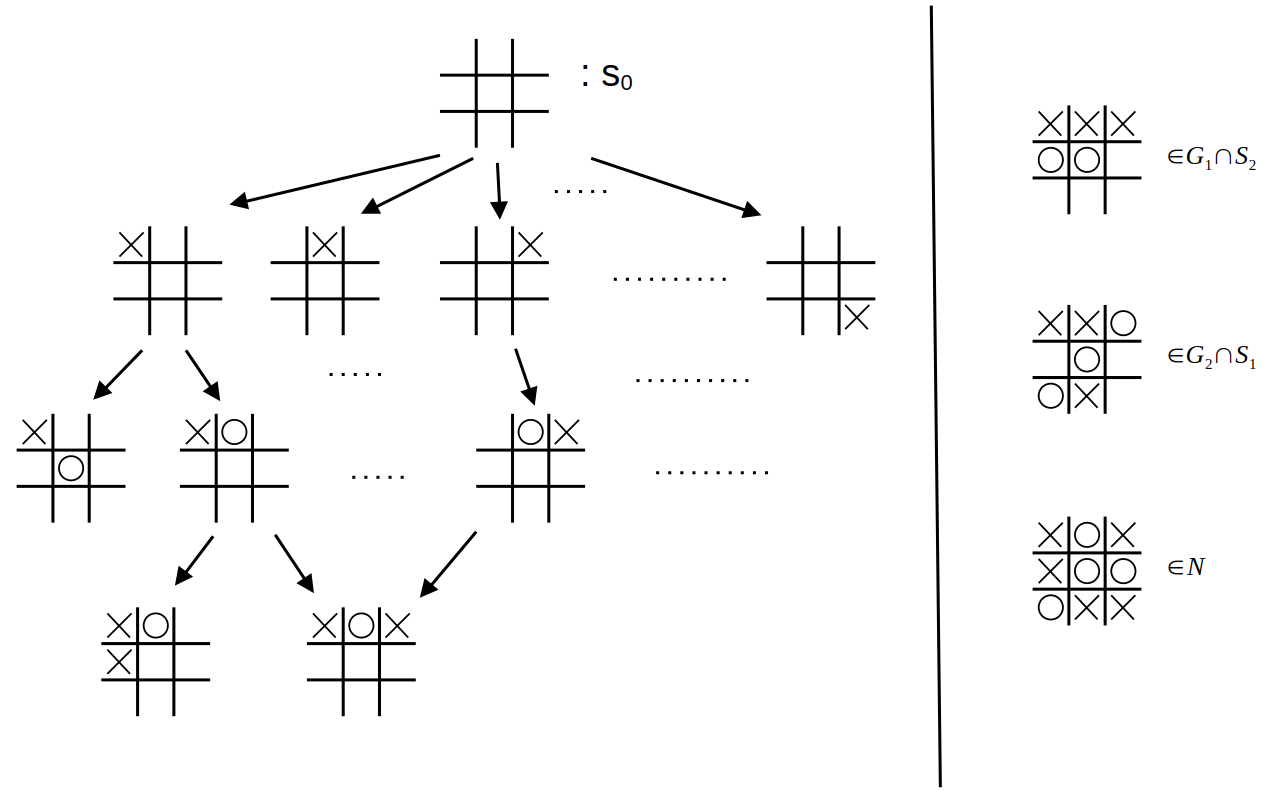
\includegraphics[width=\linewidth]{lecon/16-jeu/tic-tac-toe.png}
\end{example}

\begin{definition}[Partie]
	Une partie d'un jeu $(G, s_0, G_1, G_2, N)$ est un chemin de $s_0$ à un sommet $s_f \in Fin(G)$.
\end{definition}

\begin{definition}
	On appelle stratégie pour le joueur $i \in \{1, 2\}$ toute fonction $\varphi : V_i \to V$ tel que $\forall u \in V_i \backslash Fin(G), \, (u, \varphi(u)) \in A$.
\end{definition}

\begin{com}
	Ici on définit directement une stratégie sans mémoire, le programme se limitant à cela, et les jeux que nous considérerons ne nécessitant pas de stratégie avec mémoire.
\end{com}

\begin{definition}[Stratégie gagnante]
	$\varphi$ est une stratégie gagnante pour le joueur $i$ si pour toute partie $P = s_0, \dots, s_f$,
	$$ \Big( \forall j \in \llbracket O, f-1 \rrbracket, s_j \in V_i \implies s_{j+1} = \varphi(s_j) \Big) \implies s_f \in G_i$$
	$s$ est une position gagnante s'il existe une stratégie gagnante depuis $s$.
\end{definition}

\begin{idee}
	$\varphi$ est une stratégie gagnante si quand les coups de Ji sont ceux de $\varphi$, alors Ji gagne indépendamment de ce que joue l'autre joueur. 
\end{idee}

\subsection{Attracteurs}

On se place du point de vue du joueur 1, mais la situation est symétrique avec le joueur 2.

\begin{definition}[Attracteur]
	Pour une arène $(G, s_0)$, et $F \subset V$ on note $Attr_i(F)$, l'ensemble des sommets depuis lesquels le joueur J1 a une stratégie pour arriver dans $F$ en au plus $i$ étapes. On note $Attr(F) = \bigcup\limits_{i = 0}^{+\infty} Attr_i(F)$
\end{definition}

\begin{proposition}
	Pour un jeu $(G, s_0, G_1, G_2, N)$, $Attr(G_1)$ est l'ensemble des position gagnante de J1.
\end{proposition}

\begin{proposition}\enspace
	\begin{itemize}[label=$\bullet$]
		\item $Attr_0(F) = F$
		\item $Attr_{i+1}(F) = Attr_i(F) \: \cup \: \{u \in V_1 \, / \, \mathcal N^+(u) \cap Attr_i(F) \neq \emptyset\} \: \cup \: \{u \in V_2 \, / \, \mathcal N^+(u) \subset Attr_i(F)\} $
	\end{itemize}
\end{proposition}

\begin{proposition}
	Si $G$ est fini alors $\left( Attr_i(F) \right)$ est croissante bornée, donc stationnaire. Sa limite est alors $Attr(F)$.
	
	Une stratégie gagnante depuis $Attr(F)$ est :
	$$ \begin{array}{rcl}
		\varphi : V_1 & \to V\\
		v & \mapsto & \left\{ \begin{array}{ll}
			\omega \in \mathcal N^+(v) \cap Attr_i(F) & \text{si } v \in Attr_{i+1}(F) \backslash Attr_i(F)\\
			\omega \in \mathcal N^+(v) & \text{si } v \notin Attr(F)
		\end{array} \right.
	\end{array} $$
\end{proposition}

\paragraph{Développement :} Stratégies gagnantes pour le jeu de Nim à 1 puis plusieurs tas.

\section{Jeux Min-Max}

\subsection{Algorithme Min-Max}

On considère ici des jeux à deux joueurs, en reprenant la définition \ref{16-def-jeu} en  remplaçant la partition de $Fin(G)$ par une fonction de coût $c : Fin(G) \to \mathbb Z$.

Le joueur 1 (appelé Max ici) essaye alors de maximiser par ses coups la valeur finale, et le joueur 2 (ici Min) essaye de la minimiser.

\begin{rem}
	La partie précédente en est un cas particulier avec $c(G_1) = 1$, $c(N) = 0$ et $C(G_2) = 1$ 
\end{rem}

\begin{definition}
	Une stratégie optimale pour le joueur Max (resp. Min) est une stratégie maximisant (resp. minimisant) le coût.
\end{definition}

\begin{algo}
	On fait une recherche exhaustive de tous les coups, en prenant à chaque fois celui ayant le résultat maximum (resp.minimimum) quand Max (resp. Min) joue. Cela détermine une stratégie optimale (pour les deux joueurs).
\end{algo}

\begin{rem}
	En pratique, c'est souvent infaisable tant le graphe est gros.
	\begin{example}
		Les echecs, avec +1000 victoire blanche, -1000 victoire noire et 0 nulle, le graphe a plus de $10^44$ sommets.
	\end{example}
\end{rem}

\begin{definition}
	Une heuristique $h : V \to \mathbb Z$ est une estimation de à quoi mènerait dans le meilleur cas cette position
\end{definition}

\begin{com}
	Ici on a une définition formelle avec l'intuition de son interprétation (et donc de son usage). (une heuristique, c'est simplement une fonction $V \to \mathbb Z$)
\end{com}

\begin{example}
	La fonction qui aux échecs donne la somme de la valeur des pièces
\end{example}

\begin{idee}
	On fait l'exploration exhaustive en renvoyant l'heuristique quand on a fait suffisament d'étapes.
\end{idee}

\begin{algorithm}[H]
	\caption{$MinMax(j, prof, u)$}
	\Si{$u \in Fin(G)$ ou $prof = 0$}
		{\Retour{$h(u)$}}
	\eSi{$i == 1$}
		{$f\gets \max$}
		{$f \gets\min$}
	\Retour{$f\Big(\Big\{MinMax(3-j, \,prof-1, \,v) \enspace \big/ \enspace v \in \mathcal N^+(u)\Big\}\Big)$}
\end{algorithm}

\subsection{Élagage $\alpha$-$\beta$}

\begin{minipage}{0.5\linewidth}
	\begin{idee}
		Il n'est pas nécessaire d'explorer tout l'arbre : si je suis Min et que Max au coup d'avant peut faire 5 avec un autre coup, dès que je vois que je peux faire 1, je peux arrêter d'explorer, car je sais que Max ne fera pas ce coup.
	\end{idee}
\end{minipage} \quad \begin{minipage}{0.4\linewidth}
	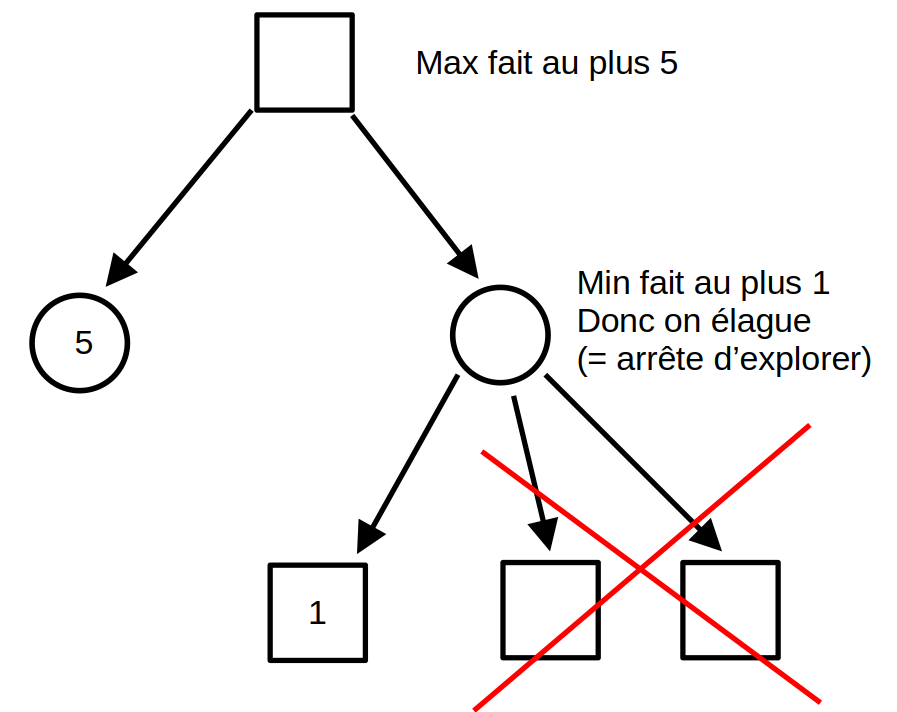
\includegraphics[width=\linewidth]{lecon/16-jeu/alpha_beta.png}
\end{minipage}

\begin{algorithm}[H]
	\caption{$Alphabeta(j, \alpha, \beta, u)$}
	\Si{$u \in Fin(G)$}
		{\Retour{$c(u)$}}
	\eSi{$joueur = 1$}
	{
		$res \gets -\infty$\\
		\Pour{$v$ voisin de $u$}
		{
			$e = Alphabeta(2, \max(res, \alpha), \beta, v)$\\
			\eSi{$e > \beta$}
				{\Retour{$e$}\quad \tcp{Élagage}}
				{$res \gets \max(e, res)$}
		}
		\Retour{$res$}
	}
	{
		\tcp{Symétrique, à faire en exercice}
	}
\end{algorithm}

\begin{idee}
	$\alpha$ (resp. $\beta$) est la valeur maximale (resp. minimale) que peut faire Max (resp. Min) parmi ce que l'on a explorer pour l'instant. (On appelle donc $alphabeta(1, -\infty, +\infty, s_0)$)
\end{idee}

\begin{rem}
	Cet algorithme est exact. On peut, comme pour Min-Max ajouter une profondeur et une heuristique.
\end{rem}

\begin{exercise}
	Comparaison des temps d'exécution de Min-Max et de Alpha-Beta pour le Tic-Tac-Toe (exploration complète sans heuristique).
\end{exercise}

\section{Les Jeux à un joueur}

\subsection{Graphe d'état}

\begin{definition}
	Un graphe d'état est la donnée d'un graphe orienté $G = (S, A)$ pondéré par $c : A \to \N$, d'un état initial $s_0$ et d'un ensemble d'états finaux $F \subset S$
\end{definition}

\begin{rem}
	$S$ représente les configurations d'un jeu à un joueur, $A$ les transitions d'une configuration à une autre en un coup, $c$ le coût de cette transition, et $F$ les configurations gagnantes. 
\end{rem}

\paragraph{Objectif :} Trouver un chemin dans ce graphe entre l'état initial et l'un des états finaux de coût total minimal.

\begin{example}
	Dans le jeu du taquin, les états correspondent aux dispositions possibles du plateau. L'état final est le plateau remis dans l'ordre. Chaque case a un degré sortant inférieur ou égal à 4 qui correspond aux déplacements possibles de la case vide (vers le haut, le bas, à gauche ou à droite). Tous les déplacements ont un coût unitaire.
\end{example}

\begin{rem}
	le graphe d'état est en général trop gros pour être stocké entièrement en mémoire. Il est donc nécessaire de mettre en place des stratégies ou des heuristiques pour orienter la recherche du chemin
\end{rem}

\subsection{L'algorithme A*}

\begin{principe}
	L'algorithme A* est une variante de l'algorithme de Dijkstra pour calculer un plus court chemin entre un sommet initial $s_0$ et un sommet final $s_f$. On visite les sommets par estimation de leur proximité à $s_f$ grâce à une fonction $f$ définie par:
	
	$f(s) = d(s) + h(s)$ où $d(s)$ est le coût d'un plus court chemin entre $s_0$ et $s$ et $h(s)$ i une estimation (heuristique) du coût entre $s$ et $s_f$
\end{principe}

\begin{example}
	dans le cas du taquin, on peut penser aux heuristiques suivantes :
	\begin{itemize}[label=$\bullet$]
		\item nombre de chiffres mal placés 
		\item somme des distances de Manhattan des cases à leur position finale
	\end{itemize}
\end{example}

\begin{algorithm}[H]
	\Entree{W la matrice de poids du graphe;
		h le tableau pour l'heuristique;
		$s_{0}$ et $s_{f}$ les sommets initiaux et finaux}
	\Sortie{la distance d'un plus court chemin de $s_{0}$ à $s_{f}$}
	
	$D \gets$ tableau initialisé à $\infty$\\
	$D[s_{0}] \gets$ 0\\
	$P \gets$ file de priorité vide\\
	Ajouter $(s_{0}, h[s_{0}])$ à $P$\\
	\Tq{$P$ non vide}{
		$(s, \_) \gets$ $extraire(P)$\\
		\Si{$s = s_{f}$}{\Retour{$D[s]$}}
		\Pour{$s'$ successeur de $s$}{
			$c \gets D[s] + W[s, s']$\\
			\Si{$c < D[s']$}{
				$D[s'] \gets c$\\
				Ajouter  $(s', c+h[s'])$ à $P$\\
			}
		}
	}
	\Retour{NonAccessible}
	\caption{Algorithme A*}
\end{algorithm}

\begin{rem}
	Si $h = 0$, on retrouve Dijkstra
\end{rem}

\begin{definition}
	Une heuristique est dite admissible si $\forall u \in S, h(u) \leq d(u)$
\end{definition}

\begin{theorem}[Correction]
	Si $h$ est admissible, alors A* renvoie la distance d'un court chemin de $s_0$ à $s_f$.
\end{theorem}

\begin{definition}
	Une heuristique est dite monotone si $\forall (u,v) \in A, h(u) \leq h(v) + w(u,v)$
\end{definition}

\begin{rem}
	Dans un graphe avec les distances euclidiennes entre nœuds, la distance à vol d'oiseau est une heuristique monotone.
\end{rem}

\begin{proposition}
	Si $h$ est monotone et $h(s_f) = 0$, alors A* est correct ($h$ est admissible) et extrait chaque noeud au plus une fois.
\end{proposition}

\paragraph{Développement :} Démonstration du théorème et de la propriété précédente.

\begin{appl}
	Calcul des itinéraires par un GPS
\end{appl}